\documentclass[12pt]{article}
\usepackage[utf8]{inputenc}
\usepackage{amsmath,amssymb,latexsym}
\usepackage{enumerate}
\usepackage{graphicx}
\usepackage{float}
\usepackage[spanish]{babel}
\usepackage{xypic}

\textheight=25cm \textwidth=18cm \topmargin=-2cm \oddsidemargin=-1cm

\newcommand{\abs}[1]{\left\vert#1\right\vert}
\newcommand{\norm}[1]{\left\Vert#1\right\Vert}

\newcommand{\Co}{\mathfrak C}
\newcommand{\F}{\mathfrak F}
\newcommand{\h}{\mathrm h}
\newcommand{\n}{\mathfrak{n}}
\newcommand{\N}{\mathbb N}
\newcommand{\Q}{\mathbb Q}
\newcommand{\R}{\mathbb R}
\newcommand{\US}{\mathbb{S}^2}
\newcommand{\x}{\mathrm x}
\newcommand{\y}{\mathrm y}
\newcommand{\z}{\mathrm z}
\newcommand{\Z}{\mathbb Z}

\newcommand{\eps}{\varepsilon}
\newcommand{\To}{\longrightarrow}
\newcommand{\mTo}{\longmapsto}

\begin{document}

\pagestyle{empty}
\begin{center}
{\textsc{Cálculo Diferencial e Integral III} \\
\medskip 
\large{Ejercicios I - 4 \\
Luis David Uicab Martínez \\
(Funciones entre espacios euclidianos)}}
\end{center}
\bigskip

\begin{enumerate}

\item Determina una pseudoparametrizaci\'on continua de la cicloide.
    \begin{figure}[H]
        \centering
        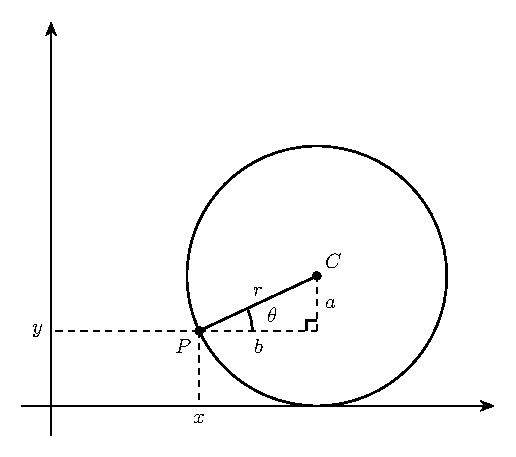
\includegraphics[width=0.4\textwidth]{Figuras (5).pdf}
    \end{figure}
    \textbf{Solución.} Sean $a,b$ como en el dibujo, $P=(x,y)$ el punto a seguir en la circunferencia de radio $r$ y $\theta$ el ángulo recorrido por el círculo. Así, 
    $a=r\cos\theta$, $b=r\sin\theta$ y en consecuencia
    \begin{align*}
        y &=r-a \\
        &=r-r\cos\theta \\
        &=r(1-\cos\theta).
    \end{align*}
    Por otra parte, definimos $s$ como la distancia que hay del origen al punto de la circunferencia tangente al eje $x$. Dicha distancia, es justamente la longitud de arco
    del sector de la circunferencia con ángulo $\theta$, de lo que se sigue $s=\theta r$. Luego,
    \begin{align*}
        x &= s-b \\
        &= r\theta-r\sin\theta \\
        &= r(\theta-\sin\theta).
    \end{align*}
    Finalmente, de las igualdades anteriores, obtenemos la siguiente pseudoparametrización de la cicloide:
    \[
        L(\theta)=\left(r(\theta-\sin\theta),r(1-\cos\theta)\right).
    \]
    \hfill $\blacktriangle$

\newpage
\item Usando las transformaciones de coordenadas cil\'indricas y esf\'ericas, determina una \emph{pseudoparametrizaci\'on} continua de: 
\begin{enumerate}[(1)]
\item El cilindro circular recto $x^2+y^2=1$, $0\leq z\leq 1$.
\item La esfera unitaria $\US$.
\end{enumerate}
\textbf{Solución.}
\begin{enumerate}[(a)]
    \item Notemos que tenemos la parametrización del círculo de radio 1, $L(t)=(\cos t,\sin t)$. Puesto que el cilindro es ir desplazando dicha circunferencia de 0 a 1,
        obtenemos la parametrización
        \[
            L_0(t,z)=\left(\cos t,\sin t, z\right).
        \]
    \item Queremos la parametrización de $x^2+y^2+z^2=1$. Transformándolo a coordenadas esféricas $x=r\sin\psi\cos\theta $, $y=r\sin\psi\sin\theta$ y $z=r\cos\psi$ se sigue que
        \begin{align*}
            1 &= r^2\sin^2\psi\cos^2\theta + r^2\sin^2\psi\sin^2\theta + r^2\cos^2\psi \\
            &= r^2\sin^2\psi(\cos^2\theta+\sin^2\theta) + r^2\cos^2\psi \\
            &= r^2(\sin^2\psi + \cos^2\psi) \\
            &= r^2.
        \end{align*}
        Así, $r=1$, y obtenemos la parametrización de la esfera unitaria
        \[
        L(\psi,\theta)=(\sin\psi\cos\theta,\sin\psi\sin\theta,\cos\psi).
        \]
        \hfill $\blacktriangle$
\end{enumerate}

\newpage
\item Determina una pseudoparametrización continua de:
\begin{enumerate}[(1)]
\item El toro bidimensional $\mathbb{T}^2$.
\item La esfera unitaria usando proyección estereográfica.
\end{enumerate}
\textbf{Solución.}
\begin{enumerate}

    \item Sean $r,R$ los radios menor y mayor del toro con centro en $(0,0,0)$. 
    \begin{figure}[H]
        \centering
        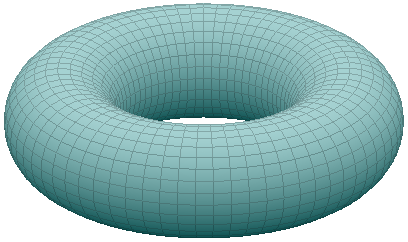
\includegraphics[width=0.4\textwidth]{Figuras (7).pdf}
    \end{figure}
    Sea $\theta$ el ángulo que genera el punto $(x_0,y_0,0)$ en la circunferencia de radio $R$ en el plano $\Pi_{xy}$.
    Sea ahora un punto $(x_1,y_1,z_1)$ en la circunferencia de radio $r$ con centro en el origen que está en el plano $\Pi_{xz}$. Luego, rotemos dicha circunferencia respecto al eje $x$, $theta$ radianes,
    y procedamos a trasladar el centro de dicha circunferencia a una distancia $R$ del centro, en el plano $\Pi_{xy}$. Así, nuestro punto $(x_1,y_1,z_1)$ tras sufrir dichas trnasformaciones, está en el toro definido al inicio.
    A este nuevo punto le llamaremos $(x,y,z)$. Notemos que la distancia del origen a $(x,y,0)$ es
    la distancia
    \[
    R+r\cos\psi.
    \]
    Así,
    \[
    x=\left(R+r\cos\psi\right)\cos\theta, \quad y=\left(R+r\cos\psi\right)\sin\theta.
    \]
    Hacemos ver que la coordenada $z$ es igual a $r\sin\psi$. De lo anterior obtenemos la parametrización
    \[
    \gamma(\theta,\psi) = \left(\left(R+r\cos\psi\right)\cos\theta,\left(R+r\cos\psi\right)\sin\theta,r\sin\psi\right).
    \]
    \item Sea $(x_1,X_2,0) \in \R^3$ arbitrario. Definamos la esfera unitaria con polo en $N=(0,0,2)$. La recta de $N$ a $(x_1,x_2,0)$ es
    \begin{align*}
        L &= \{(0,0,2)+t((x_1,x_2,0)-(0,0,2))|t\in\R\} \\
        &= \{(tx_1,tx_2,2-2t)|t\in\R\}.
    \end{align*}
    Luego, queremos encontrar los puntos $(x,y,z)\in L$ tales que $x^2+y^2+(z-1)^2=1$. Para ello notemos que
    \begin{align*}
        (tx_1)^2 + (tx_2)^2 + (1-2t)^2 = 1 &\iff t^2x_1^2 + t^2x_2^2 +1-4t+4t^2 = 1 \\
        &\iff t(tx_1^2+tx_2^2+4t-4) = 0 \\
        &\iff t=0 \text{ o } t=\frac{4}{x_1^2+x_2^2-4}.
    \end{align*}
    Notemos que la proyección estereográfica no puede mapear el punto $N$. Así, descartamos $t=0$. De ello, se sigue que la pseudoparametrización que buscamos es
    \[
        \gamma(x_1,x_2) = \left(\frac{4x_1}{x_1^2+x_2^2+4},\frac{4x_2}{x_1^2+x_2^2+4},2-\frac{8}{x_1^2+x_2^2+4}\right).
    \]
    \hfill $\blacktriangle$
\end{enumerate}

\newpage
\item Prueba que las siguientes funciones son continuas en su dominio:
\begin{enumerate}[(1)]
\item Las funciones de proyección coordenadas de $\pi_j:\R^n\To \R$ dadas por $\pi_j(x_1,\ldots,x_n)=x_j$, para cada $j=1,\ldots,n$.
\item Una función lineal $L:\R^n\To \R^m$.
\end{enumerate}
\textbf{Demostración.}
\begin{enumerate}[(b)]
    \item Sean $(x_1,...,x_n),(y_1,...,y_n) \ in \R^n$ y $\alpha$ arbitrarios. Notemos que
    \begin{align*}
        \pi_j(\alpha(x_1,...,x_n)+(y_1,...,y_n)) &= \pi(\alpha x_1+y_1,\alpha x_2+y_2) \\
        &= \alpha x_j + y_j \\
        &= \alpha \pi_j(x_1,...,x_n) + \pi_j(y_1,...,y_n),
    \end{align*}
    con lo que afirmamos, $\pi_j$ es lineal. Luego, el resultado se sigue del inciso $(b)$ de este ejercicio.
    \item Por el ejercicio 9 de esta tarea, sabemos que $L$ es uniformemente continua, y en particular, continua, de lo que se sigue el resultado. \hfill $\blacksquare$
\end{enumerate}

\item Prueba la siguiente versión del teorema del valor intermedio: Supongamos que $\Omega\subset \R^n$, $f\in \Co(\Omega,\R)$, $C\subset \Omega$ conexo y 
$\x_1,\x_2\in C$ tales que $f(\x_1)<f(\x_2)$. Si $c\in \R$ es tal que 
$f(\x_1)<c<f(\x_2)$ entonces existe $\x\in C$ tal que $f(\x)=c$. \\
\textbf{Demostración.} Puesto que $C$ es conexo, $f(C)$ es conexo.
Luego, dado que $x_1,x_2 \in C$, afirmamos que $f(x_1),f(x_2) \in f(C)$.
Así, en vistas de que $f(C)$ es conexo en $\R$, afirmamos que $f(C)$ es un intervalo. Luego,
\[
[f(x_1),f(x_2)] \subseteq f(C).
\]
Dado que $c$ está en el intervalo previamente descrito, se sigue que $c \in f(C)$ lo que nos lleva a concluir por definición de imagen, que existe $x$ tal que $f(x)=c$, de lo que se sigue el resultado. \\
\hfill $\blacksquare$


\item Supongamos que $f\in \Co(\Omega,\R^m)$ con $\Omega\subset \R^n$ cerrado y acotado. Prueba que existen $\x_1,\x_2\in \Omega$ tales que 
$\norm{f(\x_1)}\leq \norm{f(\x)}\leq \norm{f(\x_2)}$ para toda $\x\in \Omega$. \\
\textbf{Demostración.} Definamos
\[
N=\{\norm{f(\x)}:\x\in \Omega\}.
\]
Puesto que $\Omega$ es cerrado y acotado, sabemos que $f(\Omega)$ lo es. Así, $\sup(N)$ existe. Luego, notemos que existe $s_k$ tal que
\[
\sup(N)-\frac{1}{k} \leq s_k \leq \sup(N).
\]
Luego, existe $x_k$ tal que $\norm{f(x_k)}=s_k$. De ello, tenemos la sucesión $(f(x_k))_{k\geq 1}$. Luego, la sucesión de las imaǵenes bajo la función norma de la sucesión original, converge a $\sup(N)$. De ello, puesto que todas las subsucesiones convergentes de $(\norm{f(x_k)})_{\geq 1}$ convergen precisamente a $\sup(N)$, por el ejercicio 7, se tiene que
$\sup(N) \in f(\Omega)$, y en consecuencia, existe $x_0$ tal que $\norm{f(x_0)}=\sup(N)$. Así, $\norm{x}\leq \norm{x_0}$ por definición de supremo. El caso para la cota inferior es análoga, solo que construyendo una sucesión para el ínfimo. \hfill $\blacksquare$

\newpage
\item Prueba que $K\subset \R^n$ es compacto si y s\'olo si toda sucesión $(\x_k)_{k\geq 1}$ en $K$ tiene una subsucesi\'on $(\x_{k_\ell})$ que converge a un punto $\x_0\in K$. \\
\textbf{Demostración.} Probemos la suficiencia. Sea $(\x_k)_{k\geq 1}\subseteq K$. De ello se sigue que es acotada. Luego, por Bolzano-Weirstrass existe una subsucesión $(\x_k)$ convergente a $\x_0$. Esto es que para todo $\varepsilon$, existe $N$ tal que para todo $n\geq N$,
\[
    \norm{\x_n-\x_0}<\varepsilon.
\]
Así, $(\x_0)$ es punto de acumulación. En consecuencia, $x_0 \in K$ o $x_0 \in \partial K$. Como $K$ es cerrado, sabemos que $K=\text{int}K\cup \partial K$, de lo que se sigue, $k_0 \in K$. \\
Procedamos a pobrar la necesidad. Lo haremos por contrapositiva. Puesto que
$K$ no es compacto, $K$ es no acotado. Si no es acotado, para todo $M > 0$ existe $\x$ tal que $\norm{\x}\geq M$. Así, construimos la sucesión $(\x_k)_{k\geq 1}$ tal que $\norm{\x_n} \geq n$ para todo $n$. Dicha sucesión no es acotada, y por lo tanto no posee ninguna subsucesión convergente, de lo que se sigue el resultado. \hfill $\blacksquare$

\item Supongamos que $\Omega\subset \R^n$ es cerrado y acotado y 
$F:\Omega\To \R^m$ es continua e inyectiva. Prueba que la inversa de $F$, $F^{-1}:F(\Omega)\To \R^n$ es continua en $F(\Omega)$. ?`Se sigue cumpliendo esta afirmación si $\Omega$ no es cerrado? \\
\textbf{Demostración.} Puesto que $\Omega$ es compacto y $f$ continua, se sigue que $f(\Omega)$ es continua. Tomemos $C\subseteq \Omega$ cerrado (notemos que dich conjunto también es acotado). Luego, tenemos que
$\left(F^{-1}\right)^{-1}(C) =  F(C)\subseteq F(\Omega)$ será cerrado y acotado de lo que se sigue el resultado. De no ser $\Omega$ cerrado, tomemos el siguiente contraejemplo:
definamos $\Omega=[0,2\pi)$ y $F:\Omega\longrightarrow \R$ dónde $F(x)=\cos(x)$. Sabemos que $F$ es continua, y de suponer que el resultado anterior se cumple para $\Omega$ acotada más no cerrada, obtenemos que $F^{-1}$ es continua.
Luego, puesto que $F(\Omega)=\mathbb{S}^0$, cerrado y acotado, obtenemos que $F^-1(\mathbb{S}^0)$ es cerrrado y acotado, lo que es una contradicción. 
\hfill $\blacksquare$

\newpage
\item Prueba que toda función lineal $L:\R^n\To \R^m$ es uniformemente continua. \\
\textbf{Demostración.} Sea $L$ lineal. Por el ejercicio 1 de la tarea 2, existe $M>0$ tal que
\[
\norm{L(\x)} \leq M\norm{\x},
\]
para todo $\x\in\R^n$. Sea $\varepsilon > 0$ arbitrario, y $d<\varepsilon/M$. Notemos que para $\x,\y \R^n$ tales que su distancia se menor que $\delta$, por la desigualdad antes mencionada y de la linealidad de $L$,
\begin{align*}
    \norm{L(\x)-L(\y)} &=  \norm{L(\x-\y)}\\
    & < M\norm{\x-\y} \\
    &= <M\frac{\varepsilon}{M} \\
    &=\varepsilon,
\end{align*}
de lo que se sigue, $L$ es uniformemente continua. \hfill $\blacksquare$

\item Supongamos que $F:\Omega\subset \R^n\To \R^m$ es uniformemente continua y consideremos una sucesi\'on de Cauchy $(\x_k)_{k\geq 1}$ en $\Omega$. Prueba que $(f(\x_k))_{k\in \N}$ es una sucesión de Cauchy. \\
\textbf{Demostración.}
Sea $\varepsilon > 0$ arbitrario. Puesto que $f$ es uniformemente continua en $\Omega$, existe $\delta$ tal que para todo $\x,\y \in \Omega$,
\[
\norm{\x-\y} < \delta \implies \norm{f(\x)-f(\y)}<\varepsilon. \tag{1} \label{1}
\]
Luego, como $(\x_k)$ es sucesión de Cauchy, dado el $\delta$ antes mencionado, existe $N$ tal que para todo $n,m > N$,
\[
\norm{\x_n-\x_m}<\delta.
\]
De lo anterior, y de \eqref{1}
\[
\norm{f(\x_n)-f(\x_m)}<\varepsilon,
\]
con lo que damos por concluida la demostración. \hfill $\blacksquare$
\end{enumerate}

\end{document}
